\section{Updating}

\frame{\tableofcontents[currentsection]}

\begin{frame}
    \frametitle{Problem Statement}
    \begin{center} \ttfamily
         [1, 2, 3, 4, 5, 6][3] = 0
         $\downarrow$ \\[4mm]
         [1, 2, 3, 0, 5, 6]
    \end{center}
\end{frame}

\begin{frame}
    \frametitle{Updating an Array}
    \begin{center}
        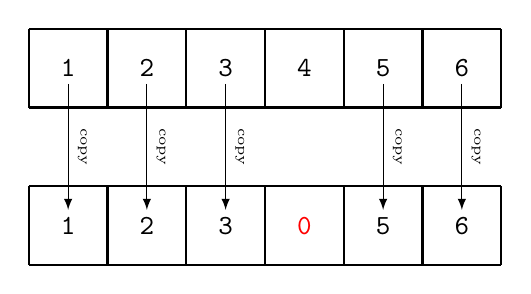
\begin{tikzpicture}
            \draw[thick] (0,0) grid ++(6,1);
            \foreach[evaluate={int(\i+1)} as \j] \i in {0,...,5} {
                \node[font=\ttfamily] at (\i + 0.5,0.5) {\j};
            }
            \foreach[evaluate={int(\i+1)} as \j] \i in {0,1,2,4,5} {
                \node[font=\ttfamily] at (\i + 0.5,-1.5) {\j};
            }
            \node[red,font=\ttfamily] at (3.5,-1.5) {0};

            \draw[thick] (0,-2) grid ++(6,1);

            \foreach \i in {0,1,2,4,5} {
                \draw[-latex] (\i + 0.5,0.3) -- (\i + 0.5,-1.3) node[midway,sloped,font=\tiny,above] {copy};
            }
        \end{tikzpicture}
    \end{center}
    \vskip4mm
    \structure{Algorithm}
    \begin{itemize}
        \item Requires copying entire array
        \item $O(n)$
    \end{itemize}
\end{frame}

\begin{frame}
    \frametitle{Updating a Linked List}
    \begin{center}
        \begin{tikzpicture}[link/.style={thick,-latex}]
            \foreach[evaluate={(\i-1) * 1.5} as \x] \i in {1,...,6} {
                \coordinate (p\i) at (\x,0);
                \llnode[position={p\i},size=0.5cm,value=\i]
            }

            \foreach[evaluate={(\i-1) * 1.5} as \x] \i/\v in {1/1,2/2,3/3,4/0} {
                \coordinate (q\i) at (\x,-1.5);
                \llnode[position={q\i},size=0.5cm,value=\v]
            }

            \foreach[evaluate={(\i-1) * 1.5} as \x] \i in {1,...,5} {
                \draw[-latex] ($ (p\i) + (0.75,0.25) $) -- ++(0.75,0);
            }

            \foreach[evaluate={(\i-1) * 1.5} as \x] \i in {1,2,3} {
                \draw[-latex] ($ (q\i) + (0.75,0.25) $) -- ++(0.75,0);
            }

            \draw[-latex] ($ (q4) + (0.75,0.25) $) -- ($ (p5) $);
        \end{tikzpicture}
    \end{center}
    \vskip4mm
    \structure{Algorithm}
    \begin{itemize}
        \item Create new list
        \item Nodes after modified element can be reused
        \item $O(n)$
    \end{itemize}
\end{frame}
